\section{Method}
\subsection{Model Architecture}
SeedProteo is a diffusion-based all-atom protein generation model specifically designed for binder design. To enable direct modeling of all-atom structures, the primary challenge lies in representing side-chain atoms when amino acid types are unknown. To address this issue, SeedProteo introduces virtual atoms and adopts the \texttt{atom14} schema \cite{quPallatomUnlockingNew2025} for all amino acids, which includes four backbone atoms and ten side-chain atoms, with virtual atoms overlaid on the C$\alpha$ atom.

As shown in Figure \ref{fig:model}, SeedProteo leverages the powerful non-equivariant atomic coordinate modeling capability of AF3-like folding model architectures, and therefore adopts a network structure consistent with such folding models: (i) an embedder module for feature initialization, (ii) an encoder composed of Pairformer blocks, and (iii) a diffusion module that denoises coordinates based on the encoder's representations.

However, a key challenge arises because the folding model's encoder is sequence-based. A trivial solution would be to replace the sequence with all \texttt{[MASK]} tokens, but such a degenerate biased input would render the encoder ineffective. To address this issue, SeedProteo additionally feeds noisy coordinates into the encoder to extract intrinsic geometric relationships: within the embedder, noisy coordinates are transformed into 1D sequence representation. This modification, however, introduces a computational cost—since the encoder, which contains cubic algorithmic complexity, becomes dependent on the noisy inputs. To mitigate the computational burden, we reduced the number of Pairformer layers from 48 to 12.

\begin{figure}[t]
    \centering
    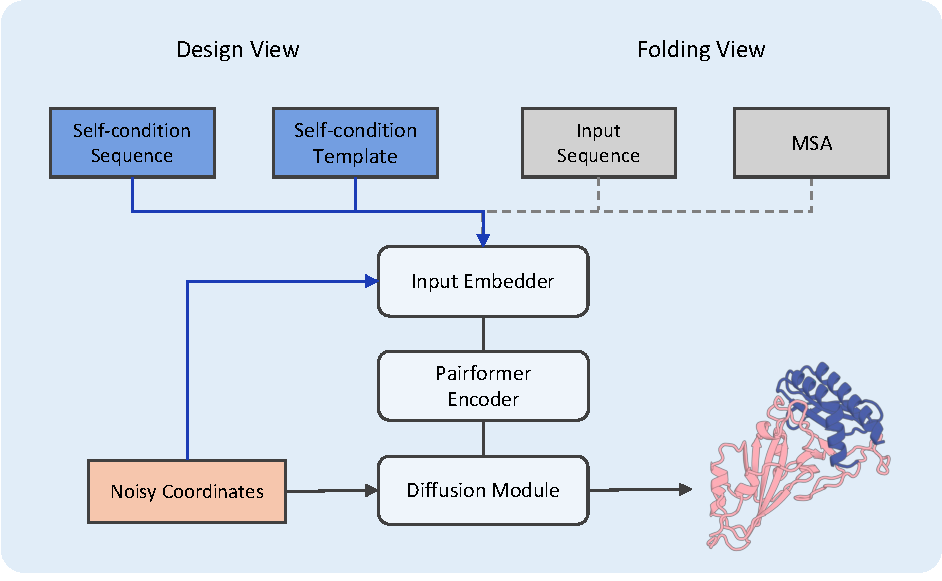
\includegraphics[width=0.75\linewidth]{figures/model.pdf}
    \caption{Overview of the SeedProteo framework. The right panel illustrates the input representation from a folding perspective. By modifying specific input channels within a nearly identical network architecture, we adapt the framework into the generative design model shown on the left.}
    \label{fig:model}
\end{figure}

\subsection{Self-conditioning features}
The distribution of protein atomic coordinates constitutes a specialized manifold. Although diffusion models can directly learn this coordinate distribution, a simple diffusion process lacking constraints often leads to the generation of structures that are geometrically plausible yet physically unrealizable. These generated backbones often exhibit poor designability, meaning that no amino acid sequence can stably fold into the generated conformation. Consequently, sequences derived from inverse folding on these structures typically fail to adopt the intended topology. Recent advances in protein design methodologies have validated the effectiveness of self-conditioning. We posit that employing effective self-conditioning features represents a promising pathway for substantially enhancing design capabilities. The following features are utilized as conditioning inputs in our model.

\begin{enumerate}
    \item \textbf{Sequence Sampling:} SeedProteo employs a Markov Random Field (MRF)-based Sequence Module \cite{renAccurateRobustProtein2024, meynardfast} to decode amino acid sequences. The probability of a sequence $\mathbf{x}$ is parameterized using the learned pair and single representations (Eq. \ref{eq:mrf}):
    \begin{equation}
    \label{eq:mrf}
        \mathrm{P}(\mathbf{X} = \mathbf{x} \mid \mathbf{a}, \mathbf{z}) 
        \propto \exp \bigg[ \sum_{i=1}^{L} h_i(x_i \mid \mathbf{a}_i) + \sum_{i=1}^{L}\sum_{j=i+1}^{L} e_{ij} (x_i, x_j \mid \mathbf{z}_{ij}) \bigg],
    \end{equation} 
    where $\mathbf{x} = (x_1, \dots, x_L)$ denotes the target amino acid sequence of length $L$, and $\mathbf{a}, \mathbf{z}$ represent the learned single and pair representations, respectively. The term $h_i(\cdot)$ models the site-specific bias for amino acid $x_i$ conditioned on the single feature $\mathbf{a}_i$, while $e_{ij}(\cdot)$ captures the pairwise coupling propensity between residues $x_i$ and $x_j$ derived from the pair feature $\mathbf{z}_{ij}$ \cite{balakrishnanLearningGenerativeModels2011}.
    We observe that this sequence-guided approach enhances the model's co-design capability by mitigating potential conflicts between sequence and structural constraints. By integrating the MRF module, SeedProteo eliminates the need to infer amino acid types by translating \texttt{atom14} coordinates. Instead, it directly utilizes the sequence inferred by the MRF, which incorporates semantic information to avoid misclassification of structurally similar (isosteric) amino acids, as the final output sequence.

    \item \textbf{Secondary Structure Sequence:} SeedProteo accepts a secondary structure (SS) sequence \cite{hekkelman2025dssp} composed of three canonical characters (H, E, L) and a special mask token (X). The model performs unmasking predictions based on the input masked SS sequence and subsequently utilizes the predicted SS sequence for self-conditioning (Eq. \ref{eq:ss_seq}):
\begin{equation}
\label{eq:ss_seq}
\begin{aligned}
    \mathcal{S}^{(0)} &= \mathcal{S}_{\text{input}}  \\
    \mathcal{S}^{(t)}_{\text{pred}} &= f_{\theta}\left(\mathcal{S}^{(t-1)}_{\text{cond}}\right)\\
    \mathcal{S}^{(t)}_{\text{cond}} &= \alpha_t \cdot \mathcal{S}^{(t)}_{\text{pred}} + (1 - \alpha_t) \cdot \mathcal{S}^{(t-1)}_{\text{cond}},
\end{aligned}
\end{equation}
% \begin{equation}
% \label{eq:ss_seq}
% \begin{aligned}
%     \mathcal{S}^{(0)} &= \mathcal{S}_{\text{input}} \quad \text{(e.g., "XXXHHXXLXEEEE")} \\
%     \mathcal{S}^{(t)}_{\text{pred}} &= f_{\theta}\left(\mathcal{S}^{(t-1)}_{\text{cond}}\right) \quad \text{(e.g., "HHHHHLLLEEEEE")}\\
%     \mathcal{S}^{(t)}_{\text{cond}} &= \alpha_t \cdot \mathcal{S}^{(t)}_{\text{pred}} + (1 - \alpha_t) \cdot \mathcal{S}^{(t-1)}_{\text{cond}}
% \end{aligned}
% \end{equation}
where $\mathcal{S}_{\text{input}}$ represents the initial, potentially masked secondary structure representation. At iteration $t$, $f_{\theta}(\cdot)$ denotes the neural network predictor parameterized by $\theta$, yielding the unmasked prediction $\mathcal{S}^{(t)}_{\text{pred}}$. This prediction is integrated into the conditioning state $\mathcal{S}^{(t)}_{\text{cond}}$ via a scalar gating factor $\alpha_t \in [0, 1]$, which controls the update rate of the self-conditioning signal.
This capability enables SeedProteo to process arbitrarily generated SS sequences, even those containing unknown segments, and adaptively refine them into a physically plausible SS sequence. We demonstrate that incorporating secondary structure features effectively guides the generation of \textit{de novo}-like structures, significantly enhancing the success rate in binder design applications.

    \item \textbf{Structural Template:} SeedProteo utilizes the denoised structure obtained from the previous step as a structural template for self-conditioning. Specifically, a binning operation is applied to convert the C$_\beta$ distance map into a one-hot tensor, which serves as a pairwise feature. We demonstrate that incorporating such template features helps stabilize the structural sampling trajectory.

\end{enumerate}

\subsection{Training Objective}
SeedProteo employs a set of loss functions commonly used in AF3-like folding models \cite{abramsonAccurateStructurePrediction2024}, including a coordinate diffusion loss, a smooth LDDT loss, and a distogram loss. The coordinate diffusion loss is applied without pre-aligning the target and predicted structures, thereby compelling the model to learn equivariance directly through this loss. Additionally, a cross-entropy loss is used to supervise the MRF-sampled sequence and the predicted secondary structure sequence.

\subsection{Training Pipeline}
SeedProteo was trained from scratch. Inspired by the training strategies of folding models, we adopted a multi-stage training pipeline. In the first stage, the model was trained using a small crop size and strictly filtered monomer data. In the second stage, training continued with a larger crop size and an expanded dataset comprising comprehensively filtered monomer data. Meanwhile, motifs are incorporated during the training process with monomer data, where partial structures paired with corresponding sequences are provided to enhance the model’s responsiveness to conditional inputs. In the third stage, the large crop size was maintained, and training proceeded with a balanced 1:1 sampling ratio of monomer data and protein multimer data. Detailed descriptions of the datasets and hyperparameters are provided in (Appendix \ref{app:data_prep} and Table \ref{tab:training_stages}).






